% -*- coding: utf-8 -*-
%-------------------------designed by zcf--------------
\documentclass[UTF8,a4paper,10pt]{ctexart}
\usepackage[left=3.17cm, right=3.17cm, top=2.74cm, bottom=2.74cm]{geometry}
\usepackage{amsmath}
\usepackage{graphicx,subfig}
\usepackage{float}
\usepackage{cite}
\usepackage{caption}
\usepackage{enumerate}
\usepackage{booktabs} %表格
\usepackage{multirow}
\newcommand{\tabincell}[2]{\begin{tabular}{@{}#1@{}}#2\end{tabular}}  %表格强制换行
\bibliographystyle{unsrt}
\usepackage{amsthm,amsmath,amssymb}
\usepackage{mathrsfs}
\usepackage{bm}
%-------------------------字体设置--------------
\usepackage{times} 
\newcommand{\yihao}{\fontsize{26pt}{36pt}\selectfont}           % 一号, 1.4 倍行距
\newcommand{\erhao}{\fontsize{22pt}{28pt}\selectfont}          % 二号, 1.25倍行距
\newcommand{\xiaoer}{\fontsize{18pt}{18pt}\selectfont}          % 小二, 单倍行距
\newcommand{\sanhao}{\fontsize{16pt}{24pt}\selectfont}  %三号字
\newcommand{\xiaosan}{\fontsize{15pt}{22pt}\selectfont}        % 小三, 1.5倍行距
\newcommand{\sihao}{\fontsize{14pt}{21pt}\selectfont}            % 四号, 1.5 倍行距
\newcommand{\banxiaosi}{\fontsize{13pt}{19.5pt}\selectfont}    % 半小四, 1.5倍行距
\newcommand{\xiaosi}{\fontsize{12pt}{18pt}\selectfont}            % 小四, 1.5倍行距
\newcommand{\dawuhao}{\fontsize{11pt}{11pt}\selectfont}       % 大五号, 单倍行距
\newcommand{\wuhao}{\fontsize{10.5pt}{15.75pt}\selectfont}    % 五号, 单倍行距
%-------------------------章节名----------------
\usepackage{ctexcap} 
\CTEXsetup[name={,、},number={ \chinese{section}}]{section}
\CTEXsetup[name={(,)},number={\chinese{subsection}}]{subsection}
\CTEXsetup[name={,.},number={\arabic{subsubsection}}]{subsubsection}
%-------------------------页眉页脚--------------
\usepackage{fancyhdr}
\pagestyle{fancy}
\lhead{\kaishu \leftmark}
% \chead{}
\rhead{\kaishu 编译原理作业报告}%加粗\bfseries 
\lfoot{}
\cfoot{\thepage}
\rfoot{}
\renewcommand{\headrulewidth}{0.1pt}  
\renewcommand{\footrulewidth}{0pt}%去掉横线
\newcommand{\HRule}{\rule{\linewidth}{0.5mm}}%标题横线
\newcommand{\HRulegrossa}{\rule{\linewidth}{1.2mm}}
%-----------------------伪代码------------------
\usepackage{algorithm}  
\usepackage{algorithmicx}  
\usepackage{algpseudocode}  
\floatname{algorithm}{Algorithm}  
\renewcommand{\algorithmicrequire}{\textbf{Input:}}  
\renewcommand{\algorithmicensure}{\textbf{Output:}} 
\usepackage{lipsum}  
\makeatletter
\newenvironment{breakablealgorithm}
  {% \begin{breakablealgorithm}
  \begin{center}
     \refstepcounter{algorithm}% New algorithm
     \hrule height.8pt depth0pt \kern2pt% \@fs@pre for \@fs@ruled
     \renewcommand{\caption}[2][\relax]{% Make a new \caption
      {\raggedright\textbf{\ALG@name~\thealgorithm} ##2\par}%
      \ifx\relax##1\relax % #1 is \relax
         \addcontentsline{loa}{algorithm}{\protect\numberline{\thealgorithm}##2}%
      \else % #1 is not \relax
         \addcontentsline{loa}{algorithm}{\protect\numberline{\thealgorithm}##1}%
      \fi
      \kern2pt\hrule\kern2pt
     }
  }{% \end{breakablealgorithm}
     \kern2pt\hrule\relax% \@fs@post for \@fs@ruled
  \end{center}
  }
\makeatother
%------------------------代码-------------------

\usepackage{xcolor} 
\usepackage{listings} 
\usepackage{fontspec}
\newfontfamily\menlo{Menlo}
\setmonofont[Mapping={}]{Monaco} 
\definecolor{mygreen}{rgb}{0,0.6,0}
\definecolor{mygray}{rgb}{0.5,0.5,0.5}
\definecolor{mymauve}{rgb}{0.58,0,0.82}
\lstset{ %
backgroundcolor=\color{white},   % choose the background color
basicstyle=\footnotesize\ttfamily,        % size of fonts used for the code
columns=fullflexible,
breaklines=true,                 % automatic line breaking only at whitespace
captionpos=b,                    % sets the caption-position to bottom
tabsize=4,
commentstyle=\color{mygreen},    % comment style
escapeinside={\%*}{*)},          % if you want to add LaTeX within your code
keywordstyle=\color{blue},       % keyword style
stringstyle=\color{mymauve}\ttfamily,     % string literal style
frame=single,
rulesepcolor=\color{red!20!green!20!blue!20},
numbers=left,
 numberstyle=\tiny\menlo
% identifierstyle=\color{red},
% language=c++,
}
%------------超链接----------
\usepackage[colorlinks,linkcolor=black,anchorcolor=blue]{hyperref}
%------------------------TODO-------------------
\usepackage{enumitem,amssymb}
\newlist{todolist}{itemize}{2}
\setlist[todolist]{label=$\square$}
% for check symbol 
\usepackage{pifont}
\newcommand{\cmark}{\ding{51}}%
\newcommand{\xmark}{\ding{55}}%
\newcommand{\done}{\rlap{$\square$}{\raisebox{2pt}{\large\hspace{1pt}\cmark}}\hspace{-2.5pt}}
\newcommand{\wontfix}{\rlap{$\square$}{\large\hspace{1pt}\xmark}}
%------------------------水印-------------------
\usepackage{tikz}
\usepackage{xcolor}
\usepackage{eso-pic}

\newcommand{\watermark}[3]{\AddToShipoutPictureBG{
\parbox[b][\paperheight]{\paperwidth}{
\vfill%
\centering%
\tikz[remember picture, overlay]%
  \node [rotate = #1, scale = #2] at (current page.center)%
    {\textcolor{gray!80!cyan!30!magenta!30}{#3}};
\vfill}}}



%———————————————————————————————————————————正文———————————————————————————————————————————————
%----------------------------------------------
\begin{document}
\begin{titlepage}
    \begin{center}
    
\includegraphics[width=0.8\textwidth]{NKU.png}\\[1cm]    
    \textsc{\Huge \kaishu{\textbf{南\ \ \ \ \ \ 开\ \ \ \ \ \ 大\ \ \ \ \ \ 学}} }\\[0.9cm]
    \textsc{\huge \kaishu{\textbf{计\ \ 算\ \ 机\ \ 学\ \ 院}}}\\[0.5cm]
    \textsc{\Large \textbf{编译原理作业报告}}\\[0.8cm]
    \HRule \\[0.9cm]
    { \LARGE \bfseries 定义你的编译器\&汇编程序}\\[0.4cm]
    \HRule \\[2.0cm]
    \centering
    \textsc{\LARGE \kaishu{朱浩泽\ 1911530}}\\[0.5cm]
    \textsc{\LARGE \kaishu{年级\ :\ 2019级}}\\[0.5cm]
    \textsc{\LARGE \kaishu{专业\ :\ 计算机科学与技术}}\\[0.5cm]
    \textsc{\LARGE \kaishu{指导教师\ :\ 王刚}}\\[0.5cm]
    \vfill
    {\Large \today}
    \end{center}
\end{titlepage}
% -------------摘------要--------------
\newpage
\thispagestyle{empty}
\renewcommand{\abstractname}{\kaishu \sihao \textbf{摘要}}
    \begin{abstract}
    \textbf{本人未进行分组,所有任务均为独立完成。此次实验主要内容为对SysY语言特性进行分析和形式化定义并设计了上下文无关文法,以及对所设计的语言进行向arm汇编程序的手写转化。}
    \\
        \noindent  %顶格
        \textbf{\\\ 关键字:}SysY语言、形式化定义、arm汇编\textbf{} \\\ \\\
    \end{abstract}
% ----------------------------------------------------------------
\tableofcontents
% ----------------------------------------------------------------
\newpage
\watermark{60}{10}{NKU}
\setcounter{page}{1}
% \section{概述}
% %——————————————————————————————————————
% \subsection{第一节}
% 如图\ref{fig:1}所示
% \begin{figure}[H]
%     \centering
%     
\includegraphics[scale=0.3]{NKU.png}
%     \caption{Caption}
%     \label{fig:1}
% \end{figure}

% 表
% \begin{table}[!htbp]
%   \centering
%   \begin{tabular}{ccccccccccc}
%   \toprule  
%   N/n$\backslash$Algo& naive-conv& naive-pool& omp-conv& omp-pool\\
%   \midrule
%   64/2& 0.0167& 0.01255& 0.04142& 0.03799\\
%   64/4& 0.03599&0.0394& 0.0458& 0.0421\\
%   \bottomrule
%   \end{tabular}
%   \caption{性能测试结果(4线程)(单位:ms)}
% \end{table}

% 带单元格表格
% \begin{table}[!htbp]
%   \centering
%   \begin{tabular}{|c|c|c|c|c|c|c|}
%   \hline
%   \multicolumn{2}{|c|}{ \multirow{2}*{$Cost$} }& \multicolumn{5}{c|}{To}\\
%   \cline{3-7}
%   \multicolumn{2}{|c|}{}&$A$&$B$&$C$&$D$&$E$\\
%   \hline
%   \multirow{3}*{From}&$B$&7&0&1&3&8\\
%   \cline{2-7}
%   &$C$&8&1&0&2&7\\
%   \cline{2-7}
%   &$D$&8&3&2&0&5\\
%   \hline
%   \end{tabular}
%   \caption{结点C距离向量表(无毒性逆转)}
% \end{table}

% %——————————————————————————————————————
% \subsection{第二节}
% 伪代码

% \begin{breakablealgorithm} 
%   \caption{初始化obj文件信息——对应MeshSimplify类中readfile函数,Face类calMatrix函数} 
%   \begin{algorithmic}[1] %每行显示行号  
%       \Require obj文件,顶点、边、面列表
%       \Ensure 是否读取成功
%       \Function {calMatrix}{$Face$}  
%               \State $normal \gets e1×e2$  
%               \State $normal \gets normal/normal.length$
%               \State $temp[] \gets {normal.x, normal.y, normal.z, normal· Face.v1}$
%               \State $Matrix[i][j]=temp[i] * temp[j]$ 
%               \State \Return{$Matrix$}  
%       \EndFunction
%       \State 根据obj的v和f区分点面信息,读取并加入列表
%       \State $scale \gets $记录点坐标中距离原点最远的分量,以便后续OpenGL进行显示
%       \State $ori \gets $记录中心点,便于OpenGL显示在中心位置,避免有的obj偏移原点较多
%       \State 根据三角面片信息,计算一个面的三条边
%       \State 计算每个面的矩阵$\gets calMatrix$
%       \State 将每个面的矩阵加到各点,由点维护\\
%       \Return True
%   \end{algorithmic}  
% \end{breakablealgorithm}

% 代码
% \begin{lstlisting}[title=逐列访问平凡算法,frame=trbl,language={C++}]
%   void ord()   
%   {
%       double head,tail,freq,head1,tail1,timess=0; // timers
%       init(N);
%       QueryPerformanceFrequency((LARGE_INTEGER *)&freq );
%       QueryPerformanceCounter((LARGE_INTEGER *)&head);
%       for (int i=0; i<NN; i++)
%           for (int j=0; j<NN; j++)
%               col_sum[i] += (b[j][i]*a[j]);
%       QueryPerformanceCounter ((LARGE_INTEGER *)& tail) ;
%       cout << "\nordCol" <<(tail-head)*1000.0 / freq<< "ms" << endl;
%   }
% \end{lstlisting}


% %——————————————————————————————————————
% \subsection{第三节}

% 参考文献\cite{adams1995hitchhiker}\cite{shin2016deep}
    
% 多行公式
% \begin{align}
%   a+b = a + b \\
%   \frac{a+b}{a-b}
% \end{align}

% 行内公式:$\sum^N_{i=1}$

% \textbf{超链接}  \href{http://youtube.com/}{YouTube}

% 带标号枚举
% \begin{enumerate}
%   \item 1
%   \item 2
% \end{enumerate}

% 不带标号枚举
% \begin{itemize}
%   \item 1
%   \item 2
% \end{itemize}

%----------------------------------------------------------------
\section{SysY语言特性和形式化定义}
\subsection{SysY语言特性}
Sysy语言是C语言的一个子集,因此继承了C语言的语法定义和特性。由函数、常变量声明、语句、表达式等多种元素构成。接下来,我们将对这种语言的每个部分的特性进行具体分析。
\subsubsection{关键字}C++常用关键字如表\ref{fig:1}所示,每一个关键字在上下文无关文法中都会看作一个终结符,即语法树的叶结点。本实验将选取其中的一部分作为子集,构造SysY语言。
\begin{table}[!htbp]
  \centering
  \begin{tabular}{ccccccccccc}
  \toprule  
  类型& 关键字&\\
  \midrule
  数据类型相关&$int,bool,true,false,char,wchar\_t,int,double,float,short,$&\\
  & $long,signed,unsigned$&\\
  控制语句相关&$switch, case, default, do, for, while, if, else,$&\\
  & $break, continue, goto$&\\
  定义、初始化相关& $const, voltile, enum, export, extern, public, protected, private,$&\\ 
   & $template, static, struct, class, union, mutable, virtual$&\\
  系统操作相关& $catch, throw, try, new, delete, friend, inline, $&\\
  & $operator, retuster, typename$&\\
  命名相关& $using, namespace, typeof$&\\
  函数和返回值相关& $void, return, sizeof, typied$&\\
  其他& $this, asm, \*\_cast$&\\
  \bottomrule
  \end{tabular}
  \caption{C++关键字}
  \label{fig:1}
\end{table}
\par
其中,由于功能相对简单,故为了满足最基本要求,我们为SysY语言选取的保留字如表\ref{fig:2}所示:
\begin{table}[!htbp]
  \centering
  \begin{tabular}{ccccccccccc}
  \toprule  
  类型& 关键字&\\
  \midrule
  数据类型相关&$int,char$&\\
  控制语句相关&$while, if, else, break, continue$&\\
  定义、初始化相关& $const$&\\ 
  系统操作相关& $new, delete$&\\
  命名相关& $using, namespace$&\\
  函数和返回值相关& $void, return$&\\
  \bottomrule
  \end{tabular}
  \caption{SysY语言关键字}
  \label{fig:2}
\end{table}
\subsubsection{变量}
\textbf{C语言中规定,将一些程序运行中可变的值称之为变量,与常量相对。}在程序运行期间,随时可能产生一些临时数据,应用程序会将这些数据保存在一些内存单元中,每个内存单元都用一个标识符来标识。这些内存单元我们称之为变量,定义的标识符就是变量名,内存单元中存储的数据就是变量的值。\cite{bl}变量可以作左值,常量则只能作为右值。变量除了与常量相同的整型类型、实型类型、字符类型这三个基本类型之外,还有构造类型、指针类型、空类型。由于在我们定义的SysY语言中,只会使用整型变量和字符变量两种变量类型,故其余几种类型不在此描述。
\paragraph{三种基本类型}
\subparagraph{整型变量}
  整型常量为整数类型$int$的数据。可分别如下表示为八进制、十进制、十六进制
    \begin{itemize}
    \item 十进制整型变量:0, 123, -1
    \item 八进制整型变量:0123, -01
    \item 十六进制整型变量:0x123,-0x88
    \end{itemize}
  \subparagraph{实型变量} 实型变量是实际中的小数,又称为浮点型变量。按照精度可以分为单精度浮点数(float)和双精度浮点数(double)。浮点数的表示有三种方式如下:
    \begin{itemize}
    \item 指明精度的表示:以f结尾为单精度浮点数,如:2.3f;以d结尾为双精度浮点数,如:3.6d
    \item 不加任何后缀的表示:11.1,5.5
    \item 指数形式的表示:5.022e+23f,0f
    \end{itemize}
  \subparagraph{字符变量} $char$用于表示一个字符,表示形式为$'$需要表示的字符常变量$'$。其中,所表示的内容可以是英文字母、数字、标点符号以及由转义序列来表示的特殊字符。如$'$a$'$\ \  $'$3$'$\ \  $'$,$'$\ \  $'$$\backslash$n$'$。
\paragraph{变量的定义} 用于为变量分配存储空间,还可为变量指定初始值。程序中,变量有且仅有一个定义。\cite{m}变量有三个基本要素:变量名,代表变量的符号;变量的数据类型,每一个变量都应具有一种数据类型且内存中占据一定的储存空间;变量的值,变量对应的存贮空间中所存放的内容。变量的定义可以以如下的形式:
\begin{lstlisting}[language = c++]
type variable_list
\end{lstlisting}
\textbf{在我们定义的SysY语言中,将支持整型变量(十进制)、字符型变量以及行主存储的整型一维数组类型。}

\subsubsection{常量}
\textbf{C语言中规定,将一些不可变的值称之为常量。}常量可以分为整型常量、实型常量、字符常量这三种常量,其形式与整型变量、实型变量、字符变量基本相同,只不过在声明时必须初始化且在程序中不可以改变其值。\textbf{在我们定义的SysY语言中,将定义整型常量(十进制)和字符型常量。}

\subsubsection{运算符和表达式}
在C语言中,运算符分为算术运算符、关系运算符、逻辑运算符、位运算符、赋值运算符、杂项运算符六大类。其中,我们所设计的SysY语言将定义以下运算符:
\begin{table}[!htbp]
  \centering
  \begin{tabular}{ccccccccccc}
  \toprule  
  运算符& 描述&\\
  \midrule
  +& 把两个操作数相加&\\
  -& 从第一个操作数中减去第二个操作数&\\  
  *& 把两个操作数相乘&\\
  /& 分子除以分母&\\
  \%& 取模运算符,整除后的余数&\\
  \bottomrule
  \end{tabular}
  \caption{算术运算符}
\end{table}
\begin{table}[!htbp]
  \centering
  \begin{tabular}{ccccccccccc}
  \toprule  
  运算符& 描述&\\
  \midrule
  ==&  检查两个操作数的值是否相等,如果相等则条件为真。& \\
  !=&   检查两个操作数的值是否相等,如果不相等则条件为真。& \\
  >&  检查左操作数的值是否大于右操作数的值,如果是则条件为真。& \\
  <&  检查左操作数的值是否小于右操作数的值,如果是则条件为真。&\\
  >=&   检查左操作数的值是否大于或等于右操作数的值,如果是则条件为真。& \\
  <=&   检查左操作数的值是否小于或等于右操作数的值,如果是则条件为真。& \\
  \bottomrule
  \end{tabular}
  \caption{关系运算符}
\end{table}
\begin{table}[!htbp]
  \centering
  \begin{tabular}{ccccccccccc}
  \toprule  
  运算符& 描述&\\
  \midrule
  \&\& &  称为逻辑与运算符。如果两个操作数都非零,则条件为真。&\\
  ||&  称为逻辑或运算符。如果两个操作数中有任意一个非零,则条件为真。&\\
  !& 称为逻辑非运算符。用来逆转操作数的逻辑状态。&\\
  \bottomrule
  \end{tabular}
  \caption{逻辑运算符}
\end{table}
\begin{table}[!htbp]
  \centering
  \begin{tabular}{ccccccccccc}
  \toprule  
  运算符& 描述&\\
  \midrule
  =& 简单的赋值运算符,把右边操作数的值赋给左边操作数。&\\
  \bottomrule
  \end{tabular}
  \caption{赋值运算符}
\end{table}
\begin{table}[!htbp]
  \centering
  \begin{tabular}{ccccccccccc}
  \toprule  
  运算符& 描述&\\
  \midrule
  \& & 返回变量的地址。&\\
  * & 指向一个变量。&\\
  \bottomrule
  \end{tabular}
  \caption{复杂运算符}
\end{table}
\paragraph{表达式}由运算分量和运算符按一定规则组成。运算分量是运算符操作的对象,通常是各种类型的数据。运算符指明表达式的类型;表达式的运算结果是一个值——表达式的值。出现在赋值运算符左边的分量为左值,代表着一个可以存放数据的存储空间;左值只能是变量,不能是常量或表达式,因为只有变量才可以带表存放数据的存储空间。出现在赋值运算符右边的分量为右值,右值没有特殊要求。
\paragraph{运算符优先级}运算符中优先级确定了表达式中项的组合,这会极大地影响表达式的计算过程以及结果。运算的优先顺序为:括号优先运算$\rightarrow$优先级高的运算符优先运算$\rightarrow$优先级相同的运算参照运算符结合性依次进行。
当表达式包含多个同级运算符时,运算的先后次序分为左结合规则和右结合规则。其中左结合规则是从左向右依次计算,包括的运算符有双目的算术运算符、关系运算符、逻辑运算符、位运算符、逗号运算符;右结合规则是从右向左依次计算,包括的运算符有可以连续运算的单目运算符、赋值运算符、条件运算符。
运算符优先级由高到低排列:后缀$\rightarrow$一元 $\rightarrow$
乘除$\rightarrow$
加减$\rightarrow$
移位$\rightarrow$ 
关系$\rightarrow$
相等$\rightarrow$
位与$\rightarrow$
位异或$\rightarrow$
位或$\rightarrow$
逻辑与$\rightarrow$
逻辑或$\rightarrow$
条件$\rightarrow$
赋值$\rightarrow$
逗号
\subsubsection{语句}
在C语言中,语句分为说明语句、表达式语句、控制语句、标签语句、复合语句和块语句。\textbf{在我们所定义的SysY语言中,我们将定义表达式语句和控制语句,其中控制语句分为分支语句、循环语句和转向语句。}
\paragraph{表达式语句} 任意有效表达式都可以作为表达式语句,其形式为表达式后面加上“;”。
\paragraph{分支语句} if语句和if……else语句,由关键字if和else组成。其基本形式如下
\begin{lstlisting}[language = c++]
if(expr){
  stmts
}
else{
  stmts
}
\end{lstlisting}
\paragraph{循环语句} 又称重复语句,用于重复执行某些语句。本实验的循环语句由while语句实现,基本形式如下
\begin{lstlisting}[language = c++]
while{
  stmts
}
\end{lstlisting}
\paragraph{转向语句} 用于从循环体跳出的break语句;用于立即结束本次循环而去继续下一次循环的continue语句;用于立即从某个函数中返回到调用该函数位置的return语句。
\subsubsection{函数}
\paragraph{函数的定义}函数是一组一起执行一个任务的语句。程序中功能相同,结构相似的代码段可以用函数进行描述。函数的功能相对独立,用来解决某个问题,具有明显的入口和出口。函数也可以称为方法、子例程或程序等等。
\paragraph{函数说明}
C语言中,函数必须先说明后调用。函数的说明方式有两种,一种是函数原型,相当于“说明语句”,必须出现在调用函数之前;一种是函数定义,相当于“说明语句+初始化”,可以出现在程序的任何合适的地方。在函数声明中,参数的名称并不重要,只有参数的类型是必需的。函数的声明形式如下所示:
\begin{lstlisting}[language = c++]
return_type function_name(parameter list);
\end{lstlisting}
\paragraph{形式化定义}C语言中,函数的形式化定义如下所示:
\begin{lstlisting}[language = c++]
return_type function_name(parameter list)
{
   body of the function
}
\end{lstlisting}
\textbf{本实验定义的SysY语言的函数定义完全与此相同。}
\paragraph{函数的参数}
函数可以分为有参函数和无参函数。如果函数要使用参数,则必须声明接受参数值的变量,这些变量称为函数的形式参数。形式参数和函数中的局部变量一样,在函数创建时被赋予地址,在函数退出是被销毁。函数参数的调用分为传值调用和引用调用两种,传值调用是将实际的变量的值复制给形式参数,形式参数在函数体中的改变不会影响实际变量;引用调用是将形式参数作为指针调用指向实际变量的地址,当对在函数体中对形式参数的指向操作时,就相当于对实际参数本身进行的操作。\\
\\
除此之外,函数还可以分为内联函数、外部函数等等,并还可以进行重载等操作。\textbf{本次实验的SysY语言,只对函数最基本的功能进行实现。}
\subsection{形式化定义}
接下来,我们将采用CFG即上下文无关文法对SysY语言进行形式化定义。上下文无关文由一个终结符号集合$V_T$、一个非终结符号集合$V_N$、一个产生式集合$\mathscr{P}$和一个开始符号$S$四个元素组成。在接下来的定义中,数位、符号和黑体字符串将被看作终结符号,斜体字符串将被看作非终结符号。若多个产生式以一个非终结符号为头部,则这些产生式的右部可以放在一起,并用|分割。
\begin{table}[!htbp]
  \centering
  \begin{tabular}{ccccccccccc}
  \toprule  
  名称& 符号& 名称& 符号&\\
  \midrule
  声明语句& $decl$& 标识符& $\tt{id}$\\
  标识符列表& $idlist$&数据类型& $type$\\
  表达式&$expr$&一元表达式&$unary\_expr$\\
  赋值表达式&$assign\_expr$&逻辑表达式&$logical\_expr$\\
  算数表达式&$math\_expr$&关系表达式&$relation\_expr$\\
  数字&$\tt{digit}$&整数&$decimal$\\
  符号和字母&$\tt{character}$&常量定义&$const\_init$\\
  分配内存& $allocate$& 回收内存& $recovery$\\
  语句& $stmt$& 循环语句& $loop\_stmt$\\
  分支语句& $selection\_stmt$& 跳转语句& $jmp\_stmt$\\
  函数定义& $funcdef$& 函数参数& $para$\\
  函数参数列表& $paralist$& 函数名称& $funcname$\\
  函数返回值& $re\_type$\\
  \bottomrule
  \end{tabular}
  \caption{下文中各符号含义}
\end{table}


\subsubsection{变量声明}
变量可以声明分为仅声明变量和声明变量且赋初值。(整型变量只支持十进制)数组由指针实现。
\begin{align*}
idlist \rightarrow\ & idlist,\tt{id}\ |\ \tt{id}\\
type \rightarrow\ & \tt{int} \ | \ \tt{char}\\
decl \rightarrow\ & type\ idlist \ | \\
&type\ \text{$\tt{id}$} = logical\_expr \ |\\
&type\ \text{$\tt{id}$} = unary\_expr \ | \\
&type \ *\text{$\tt{id}$} = \tt{\&id}
\end{align*}
\subsubsection{常量声明}
常量包括整型常量(十进制)和字符型常量。
\begin{align*}
const\_init\rightarrow\ \tt{const}\ \it{type}\ \tt{id} = \it{unary\_expr}
\end{align*}
\subsubsection{表达式}
表达式可以分为一元表达式、赋值表达式、逻辑表达式、算数表达式、关系表达式。
$$
expr \rightarrow \ unary\_expr \ |\ assign\_expr \ |\ logical\_expr \ |\ math\_expr \ |\ relation\_expr
$$
\subsubsection{赋值表达式}
赋值表达式不能对常量进行赋值。
\begin{align*}
\tt{digit}\rightarrow\  &\tt{0}\ | \ \tt{1}\ | \ \tt{2}\ | \ \tt{3}\ | \ \tt{4}\ | \ \tt{5}\ | \ \tt{6}\ | \ \tt{7}\ | \ \tt{8}\ | \ \tt{9}\\
decimal \rightarrow\  &\tt{digit}\ | \ \text{$decimal$}\ \tt{digit}\\
\tt{character} \rightarrow \ &\tt{\_ \ |\ a-z \ |\ A-Z}\\ 
unary\_expr \rightarrow \ &decimal \ |\ '\tt{character}' \ |\ \tt{id}\\
assign\_expr \rightarrow \ &\text{$\tt{id}$} = unary\_expr \ | \\ 
&\text{$\tt{id}$} = logical\_expr\ | \\
&\text{$\tt{id}$} = funcnmae(paralist)
\end{align*}
\subsubsection{逻辑表达式}
逻辑表达式包括逻辑与、逻辑或、逻辑非运算。
\begin{align*}
logical\_expr \rightarrow\ &unary\_expr\ |\\
&!(logical\_expr)\ |\\
&logical\_expr || logical\_expr\ |\\
&logical\_expr \&\& logical\_expr
\end{align*}
\subsubsection{关系表达式}
关系表达式包括判断两个值是否相等或比较两值的大小。
\begin{align*}
relation\_expr \rightarrow \ &unary\_expr==unary\_expr\ |\\
&unary\_expr\ != unary\_expr\ |\\
&unary\_expr > unary\_expr\ |\\
&unary\_expr < unary\_expr\ |\\
&unary\_expr >= unary\_expr\ |\\
&unary\_expr <= unary\_expr\\
\end{align*}
\subsubsection{算数表达式}
算数表达式包括加、减、乘、除、取模、取负六种运算。
\begin{align*}
math\_expr \rightarrow \ &unary\_expr\ |\\
&-unary\_expr\ |\\
&math\_expr + math\_expr\ |\\
&math\_expr - math\_expr\ |\\
&math\_expr * math\_expr\ |\\
&math\_expr\ / \ math\_expr\ |\\
&math\_expr\ \% \ math\_expr\\
\end{align*}
\subsubsection{系统操作}
系统操作包括分配内存和回收内存。
\begin{align*}
allocate \rightarrow \ &type\ \tt{*id} = \text{$\tt{new} $}\ \it{type}\ [\text{$\tt{id}$}]\ |\\
&type\ \tt{*id} =  \tt{new}\ \it{type}\ [decimal]
\end{align*}
\subsubsection{语句}
语句包括循环语句、分支语句、跳转语句。
\begin{align*}
stmt\rightarrow\ &loop\_stmt \ |\ selecion\_stmt \ |\ jmp\_stmt \ |\\ 
&expr;\ stmt\ | \\
&expr\ 
\end{align*}
\subsubsection{循环语句}
循环语句利用while实现。
$$
loop\_stmt \rightarrow \ \tt{while}\it{(expr)}\ \it{\{stmt\}}
$$
\subsubsection{分支语句}
分支语句利用if else实现。
\begin{align*}
selection\_stmt \rightarrow &\tt{if}(\it{expr})\ \{stmt\} \ | \\
&\tt{if}(\it{expr})\ \{stmt\}\ \tt{else} \ \it{\{stmt\}}
\end{align*}
\subsubsection{跳转语句}
跳转语句包括继续执行循环、退出循环和返回值。
\begin{align*}
jmp\_stmt \rightarrow\ &\tt{continue}\ |\\
&\tt{break} \ |\\
&\tt{return} \ |\\
&\tt{return}\ \it{expr}
\end{align*}
\subsubsection{函数} 
函数的返回值有整型、字符型、指针型三种,参数有整型、字符型、指针型、引用四种。(数组由指针实现)
\begin{align*}
funcdef \rightarrow\ &re\_type\ \tt{funcname}\it{(paralist)\ stmt}\\
paralist \rightarrow\ & para, paralist \ |\ para\\
para \rightarrow\ &type\ \tt{id}\ | \\
&type* \ \tt{id}\ | \\
&type\& \ \tt{id}\ \\
re\_type \rightarrow \ &type\ |\ type*\ |\ \tt{void}
\end{align*}
\subsubsection{注释}
本实验定义的SysY语言将使用//作为注释开始的符号,/*\ */将不被使用。在编译的预处理阶段,//后到行末的内容将被删除。
\subsubsection{输入输出流}
输入输出流将由SysY语言提供的I/O函数实现,在此不再定义。
%----------------------------------------------------------------
\newpage
\section{汇编编程}
本人在Linux ubuntu 4.15.0-142-generic环境下,利用vim将C++文件手动翻译成汇编文件。通过\fbox{arm-linux-gnueabihf-g++ 汇编文件名.S -o 目标文件名 -static}指令生成可执行程序,再通过\fbox{qemu-arm ./目标文件名}指令进行运行调试,最终对C++文件到arm源文件的转换有了一定的了解。手动编写的汇编文件已经上传于gitlab,链接如下:\\
\href{git@gitlab.eduxiji.net:nku2021-anthony/compilers.git}{SSH: git@gitlab.eduxiji.net:nku2021-anthony/compilers.git}\\
\href{https://gitlab.eduxiji.net/nku2021-anthony/compilers.git}{HTTP:  https://gitlab.eduxiji.net/nku2021-anthony/compilers.git}
\subsection{一些基本操作}
\subsubsection{关于函数的栈指针操作}
在现如今的计算机体系结构中,栈是向下增长的,即由大端地址增长到小端地址。在arm汇编中,fp寄存器用作帧指针,sp寄存器指向栈顶,在跳转语句调用子函数时会将当前的PC保存在lr寄存器中。当调用一个函数时,该函数首先将 fp 的当前值保存在堆栈上。然后,它将 sp 寄存器的值保存在 fp 寄存器中。然后递减 sp 寄存器来为本地变量分配空间。fp 寄存器用于访问本地变量和参数,局部变量位于帧指针的负偏移量处,传递给函数的参数位于帧指针的正偏移量。
当函数返回时,fp 寄存器被复制到 sp 寄存器中,这将释放用于局部变量的堆栈,函数调用者的 fp 寄存器的值由pop从堆栈中恢复。\cite{zhn}
\begin{lstlisting}[title = 函数被调用时的基本框架]
push {fp, lr} @将fp的当前值保存在堆栈上,然后将sp寄存器的值保存在fp中,lr中存储的是pc的保存在lr中
@被调用的函数体
pop {fp, lr} 
bx lr @相当于mov pc, lr   恢复上下文
\end{lstlisting}
\subsubsection{I/O操作}
已知在arm汇编架构中,关于C++文件输入输出流cin、cout没有直接相对应的指令,所以我们将会调用从C语言中继承的scanf和printf在其中使用。已知,在调用这两个函数时,r0寄存器保存的是自定义字符串的地址,r1寄存器保存的是“\%d”中将要被替换的内容,具体代码如下:
\begin{lstlisting}[title = arm汇编语言中的输入流模版]
sub sp, sp, #4 @在栈中开辟一块大小为4的内存地址,用于存储即将输入的数据
ldr r0, =_cin
mov r1, sp @将sp的值传输给r1寄存器,使scanf传入的值存储在栈上,即栈顶的值是输入的值
bl scanf
ldr 任意寄存器, [sp, #0] @取出sp指针指向的地址中的内容,即栈顶中的内容(输入的值)
add sp, sp, #4 @恢复栈顶,释放内存空间

.data @数据段
_cin 
  .asciz "%d"
\end{lstlisting}
\newpage
\begin{lstlisting}[title = arm汇编语言中的输出流模版]

ldr r0, =_bridge
mov r1, 要输出内容所在寄存器 
bl printf

.data
_bridge:
  .asciz "%d\n"
\end{lstlisting}
\subsection{汇编程序编写}
\subsubsection{斐波那契数列}
\begin{lstlisting}[title = 源程序, language = c++]
#include <iostream>
using namespace std;
int main()
{
    int a, b, i, t, n;
    a = 0;
    b = 1;
    i = 1;
    cin >> n;
    cout << "a:" << a << endl;
    cout << "b:" << b << endl;
    cout << "we are going to loop now! " << endl;
    while (i < n)
    {
        t = b;
        b = a + b;
        cout << b << endl;
        a = t;
        i = i + 1;
    }
    return 0;
}
\end{lstlisting}
\begin{lstlisting}[title = 改写后的汇编代码]
  .arch armv7-a @处理器架构
  .arm
@r0是格式化字符串,r1是对应的printf对应的第二个参数
@代码段
@主函数
  .text @代码段
  .global main
  .type main, %function
main: 
  push {fp, lr} @将fp的当前值保存在堆栈上,然后将sp寄存器的值保存在fp中,lr中存储的是pc的保存在lr中
  sub sp, sp, #4 @在栈中开辟一块大小为4的内存地址,用于存储即将输入的数据
  ldr r0, =_cin
  mov r1, sp @将sp的值传输给r1寄存器,使scanf传入的值存储在栈上,即栈顶的值是n
  bl scanf
  ldr r6, [sp, #0] @取出sp指针指向的地址中的内容,即栈顶中的内容(输入的n的值)
  add sp, sp, #4 @恢复栈顶,释放内存空间

  @测试是否写入
  @ldr r0, =_bridge3
        @mov r1, r2
        @bl printf

  mov r4, #0 @a = 0
  mov r5, #1 @b = 1
  mov r7, #1 @i = 1
  @r4中存a的值,r5中存b的值,r7中存i的值,r6中存n的值
  ldr r0, =_bridge
  mov r1, r4 @将r4中的值即a的值赋予r1
  bl printf @打印a的值
  ldr r0, =_bridge2
  mov r1, r5 @将r5中的值即b的值赋予r1
  bl printf @打印b的值
        ldr r0, =_bridge4
        bl printf
  
  @输出进行调试
  @ldr r0, =_bridge3
        @mov r1, r6
        @bl printf
        @ldr r0, =_bridge3
        @mov r1, r7
        @bl printf

Loop:
  @输出进行调试
  @ldr r0, =_bridge4
  @bl printf
  @ldr r0, =_bridge3
  @mov r1, r6
        @bl printf
  @ldr r0, =_bridge3
        @mov r1, r7
        @bl printf

  cmp r6, r7
  ble RETURN @比较r7和r6(即i和n)的大小用于跳转
  mov r8, r5 @t = b @r8为临时变量的寄存器
  add r5, r5, r4 @b = a + b
  ldr r0, =_bridge3
  mov r1, r5 @将r5中的值即b的值赋予r1
  bl printf  @cout << b << endl;
  mov r4, r8 @a = t
  add r7, r7, #1 @i = i + 1
  b Loop

RETURN:
  pop {fp, lr} @上下文切换
  bx lr @return 0
.data @数据段
_cin:
  .asciz "%d"

_bridge:
  .asciz "a:%d\n"

_bridge2:
  .asciz "b:%d\n"

_bridge3:
        .asciz "%d\n"

_bridge4:
  .asciz "We are going to loop now! \n"

.section .note.GNU-stack,"",%progbits @ do you know what's the use of this :-)
\end{lstlisting}
运行后的结果如图\ref{fig:1}所示。可以看出,手写汇编代码正确。
\begin{figure}[H]
    \centering
    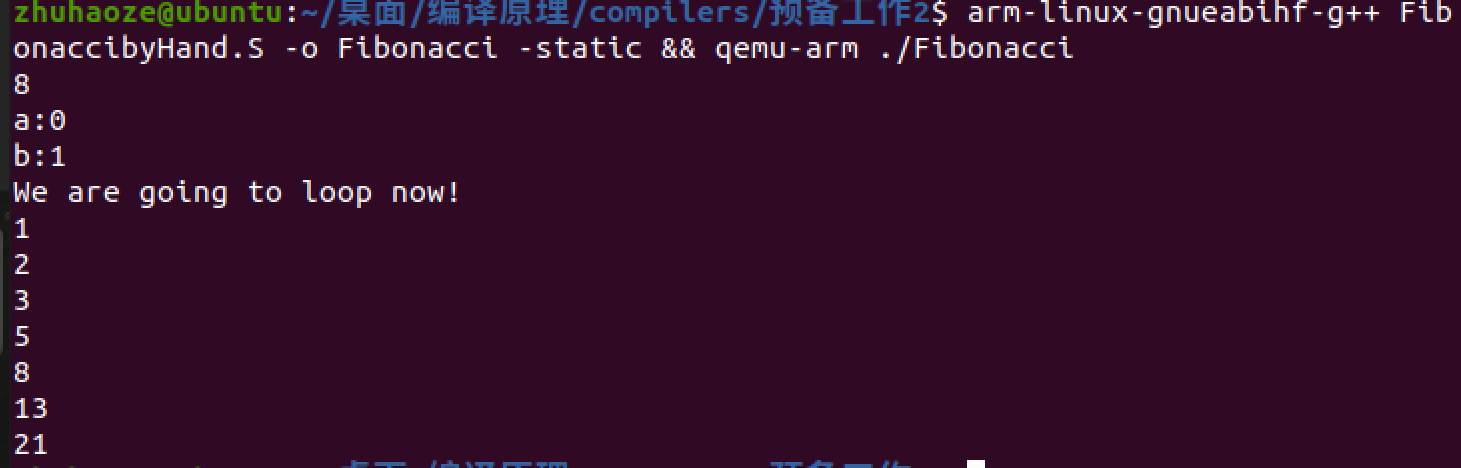
\includegraphics[scale=0.55]{1.png}
    \caption{斐波那契程序运行结果}
    \label{fig:1}
\end{figure}
\subsubsection{求平方}
\begin{lstlisting}[language = c++, title = 源程序]
#include <iostream>
using namespace std;
int square(int a){
        int m;
        m = a * a;
        return m;
}
int main()
{
        int a, s_a;
        cin >> a;
        s_a = square(a);
        cout << s_a << endl;
        return 0;
}
\end{lstlisting}
\begin{lstlisting}[title = 改写后的汇编代码]
.arch armv7-a
  .arm

  .text @代码段
  .global square
square: @function int square(int a)
  str fp, [sp, #-4]! @pre-index mode, sp = sp -4, push fp
  mov fp, sp
  sub sp, sp, #8 @为本地变量开辟空间
  str r0, [fp, #-8] @r0 = [fp, #-8] = a
  mul r1, r0, r0
  mov r0, r1
  add sp, fp, #0
  ldr fp, [sp], #4
  bx lr

  .text @代码段
  .global main
  .type main, %function
main:
  push {fp, lr}
  sub sp, sp, #4
  ldr r0, =_cin
  mov r1, sp
  bl scanf
  ldr r0, [sp, #0] @取出输入的内容放入r0中
  add sp, sp, #4
  bl square
  mov r1, r0
  ldr r0, =_cout
  bl printf
  mov r0, #0
  pop {fp, lr}
  bx lr

.data @数据段
_cin:
  .asciz "%d"

_cout:
  .asciz "%d\n"

.section .note.GNU-stack,"",%progbits @ do you know what's the use of this :-)

\end{lstlisting}
运行后的结果如图\ref{fig:2}所示。可以看出,手写汇编代码正确。
\begin{figure}[H]
    \centering
    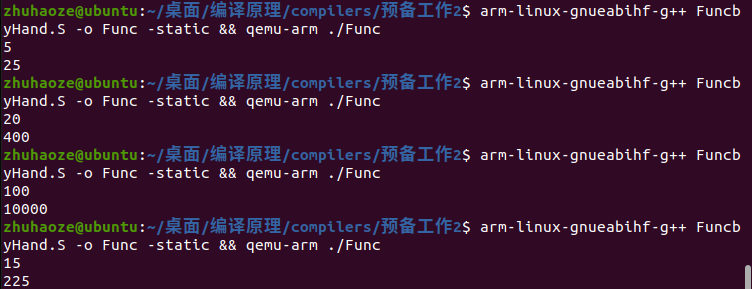
\includegraphics[scale=0.5]{2.png}
    \caption{求平方程序运行结果}
    \label{fig:2}
\end{figure}
%---------------------------------------------------------------
\vspace*{300pt}
\bibliographystyle{plain}
\bibliography{references} 
\end{document}
